\chapter{Discussion}
\label{ch:discussion}
\acresetall

\section{System Design Vulnerability/Attacks on the routing announcements?}
The design was changed a bit during implementation, and because lack of time
there was a crucial part that did not make it to the implementation, which needs
to be addressed before the system can be used in a real world scenario. There
are two attacks that the system are still vulnerable to, namely the
\emph{wormhole attack} and the \emph{suppress replay attack}.

Because the routing announcements are unencrypted and the one-time-passwords
are just appended after the messages, these packets can be altered using the
following two attacks. In this section the two attacks are first explained, and
then the section goes on to describe possible solutions for both attacks.

\subsection{Wormhole Attack}
In a wormhole attack, see Figure \ref{fig:wormhole_attack}, an attacker does not
need to know the keystream of a node in order to send that node's routing
announcements. If you look at the figure from the background chapter you have a
network of trusted nodes in green, and two malicious nodes in red. 

Assume the two attackers, M1 and M2, want to disrupt the network topology by
having node B believe node A (and vice versa) is a direct neighbor. Assuming the
out-of-band wormhole in the figure is a faster route between node A and B than
the ``real'' route through the network, M1 can simply forward the announcements
from A to M2. Then M2 does the same, except he also needs to spoof his network
and link layer addresses. When B receives the routing announcement from M2, he
believes it is from A and that A is a new direct neighbor.

Now B will ask for A's keystream-material, and M2 and M1 will forward this
request to A, which will dutifully reply with his keystream-material. Note that
M1 needs to spoof B's addresses here, as well as forwarding B's routing
announcements. When B receives the keystream through the wormhole, he is now
able to verify the routing announcements also sent through the wormhole, and
soon will this route take priority in his routing table as a strong direct link
instead of going through other nodes in the network to reach A.

TODO: MSC FIGURE VISER DETTE

This attack only distorts the network topology, but notice that because the
routing announcements' integrity are not protected, and the content is not
encrypted, the attackers can possibly do greater damage by altering the content
of the message. By altering the content, they could possibly generate fake
re-broadcast announcements announcing untrusted nodes, possibly connecting a
whole network of malicious nodes to this trusted network. This alteration is
not actually a wormhole attack, but it is fair to say that the wormhole attack
opens up to a variety of other attacks, such as alteration of packet, dropping
of packets etc.

\subsection{Suppress Replay Attack}
Another attack which is possible due to the fact that the one time passwords are
not ``connected'' to the routing announcements in any way is the suppress replay
attack. Suppose an attacker is able to jam the signals for a very short time,
only enough to distort the main payload of the routing announcement, while the
one time password and its sequence number are kept intact.

The trusted receiver of this distorted packet will ignore it, because he will
not understand the meaning of the packet. The attacker on the other hand, knows
that the following uncorrupt data is a valid one time password and its sequence
number from the sender's keystream.

Because the original recipient of this packet did not understand the destroyed
packet, he will not know that this \ac{OTP} is already used, and if the attacker
wishes to create a false routing announcement he can now do this and append the
\ac{OTP}, which will be accepted by the original recipient. Note that also here
the attacker needs to spoof the addresses of the original sender of the
announcement which he partly jammed.

\subsection{Possible Solution to the Suppress Replay Attack}
A possible solution to the suppress replay attack, is to ensure message
intergrity in addition to the authentication. The basic idea would be to create
and append a message digest to the announcement while using the keystream to
encrypt the message, e.g. by using a strong stream cipher.

There is one great pitfall to this idea, however. Because the routing
announcements are often identical to each other, the attacker might be able to
do a known plaintext attack, being able to first recreate the message digest,
and depending on the stream cipher just XOR the announcement and digest with the
encrypted message, revealing the keystream used by the stream cipher. If this
message was in any way blocked from reaching the intended recipient, the packet
could be changed and XOR'ed with the retrieved keystream and sent to the
recipient, which would trust this packet.

One possible way to avoid this problem would be to add some randomness to the
``known part'', namely the original announcement. If the announcement is e.g.
appended with a part of the senders keystream (\ac{OTP}) before creating the
message digest, the attacker would not be able to recreate the full plaintext
(including digest) and would therefore not be able to find the keystream used by
the stream cipher.

The reader might rise another question, regarding the lenght of this random part
added to the announcement before creating the digest. One major factor here is
time, and time it takes for an adversary to find the random part (collision).
The time is however very restricted. The sliding window used to avoid replay
attacks is only 64 bits long, and in the worst case (best case for adversary)
there are only two legitimate nodes in the network. If this is the case, each
node will send two announcements every second (BATMAN protocol) meaning the
window of opportunity for the attacker is only 32 seconds. For each extra
legitimate node in the network this window drastically closes. The length of the
random part used for the digest should therefore be strong enough withstand 32
seconds of brute-force guessing attack.

Note that it might not be wise to send the whole message digest because the
announcement sizes would become very large. This might be truncated as well, but
when designing this the time needed to find a collision for a truncated digest
needs to be addressed as well.

\subsection{Possible Solution to the Wormhole Attack}
This attack vector is very difficult to to protect against. With the solution
above, many attacks dependent on the wormhole attack are thwarted because of
packet secrecy, integrity and authentication. However, the solution does not
hinder an attacker from replaying the exact same packets through a wormhole, in
order to alter the network topology. There has been alot of research effort to
find a good solution to this attack, but most solutions are aimed towards
stationary networks and not \acp{MANET} \cite{raoteapproaches}.

One possible solution as pointed to by the article above is the use of
``location aware guard node'' and graph theory \cite{poovendran2007graph}
\cite{lazos2005preventing} to detect wormholes. The idea is that if you have
special nodes spread out in the field at fixed points, where none of these nodes
are within each other's transmitting range, one should never be a neighbor of
more than one node at a time. If you receive direct packets from two nodes
within a very short timeframe, there might be indications that there's a
wormhole in place replaying one of the special nodes' announcements.

\section{Key Usage}
In the fields of information security and cryptography it is not seen as a good
practice to use the same keys for different type of tasks such as encryption 
for confidentiality and signing for integrity and authenticity.

It is argued that using only one key for different purposes brings a single
point of failure to the design. While this is true, sometimes the benefits of
having single key for these purposes are greater than the risk. In the proposed
design the same public key pair is used to digitally sign keystream-material
messages as well as when encrypting (with recipients public key) the symmetric
keys in the same messages. In addition, the \acp{SP} use the same key to sign
other nodes' \acp{PC}.

The benefits of only having a singe public key pair for each node in the network
is simplicity in the design. When it comes to the possible vulnerability if the
one key is compromised, the lifetime of each key which is bound by the
relatively short lifetime of \acp{PC} makes the window of opportunity for misuse
of this key short and damage low.

\section{Extending the System Design}
The specialization project\footnote{} this thesis mentioned other important
features the secure ad hoc network implementation should have. The things
mentioned in this thesis' system design are actually implemented, but there are
still much more that should be added if this system should be used in real life
emergency situations.

In this section some important features which should be added, or at least
studied, are mentioned. They do add more complexity to the system, so it is
probably better to do a complete security and performance analysis on this
thesis' proposed design before adding these features, however.

\subsection{Initial Authentication with Long-Lived Public Key Certificates}
One limiting factor in the system design is the need for an out-of-band
initial authentication. With this limitation, every actor in the emergency
scenario needs to manually verify his or hers identity to the network management
handled by the \ac{SP}. With many actors, which would be typical in a large
emergency situation like a natural disaster, this process might take up valuable
time from the actual emergency work - which contradicts the whole meaning of
setting up the \ac{MANET} at the scene in the first place.

Now, if an actor has possession of a regular \ac{LLPKC} for which the network
\ac{SP} is able to verify, this should be allowed without the need of an
out-of-band authentication. After the \ac{SP} have verified the certificate, he
can now issue the the actor a proxy certificate, signed by him so that all nodes
in the network are able to verify the new nodes identity.

The question of whether the \ac{SP} is able to verify the \ac{LLPKC} is not
necessarily easy to answer. If the \ac{SP} trusts the identity and knows the
public key of the issuer of the actor's certificate, he is able to verify that
this actor was trusted with this identity (and rights) at some time. However, it
does not mean this is true anymore - the certificate might have been revoked.

In the absence of Internet access, \acp{CRL} might not be available to the
\ac{SP}. If this is the case, an evaluation of what to do with the actor has to
be done. Ideas that comes to mind might be to issue a very short lived \ac{PC},
maybe with limited rights, to the actor's node so that it can start working now,
but has to re-authenticate later when \acp{CRL} has been brought to the scene
either out-of-band or by setting up Internet access. If no \ac{CRL} is ever
brought to the SPs attention, he might want to require an out-of-band
authentication later.

Either way, as this does not have to happen in the same out-of-band fashion as
the proposed design in this thesis requires, one could also allow the
authentication happen even if the actor is not a direct neighbor of the \ac{SP},
but is connected through other nodes in the network.

While in this implementation regular trusted nodes drop the announcements from
new unauthenticated nodes, they could rather tunnel the announcement directly to
the \ac{SP} and have the authentication handshake go through them.

\subsection{Network Merging}
For this implementation to be really useful for emergency services, which will
consist of different types of actors and organizations, the implementation
should support merging of multiple ad hoc networks. For example, if paramedics
set up their own network, and firefighters arrive with their own network,
co-operation between these networks should be supported.

Figure \ref{fig:scenario_networks} (from the specialization
project\footnote{A.G. Bowitz and E.G. Graarud \textit{Developing a Secure Ad
Hoc Network Implementation}
\url{http://org.ntnu.no/batman2010/project_final.pdf}}) shows a possible
scenario when a large emergency situation such as a natural disaster has
happened. The figure portrays 4 organizational actors, i.e. police,
firefighters, paramedics, and the military, which all run their own networks.
Some of the networks co-operate through the use of gateways, such as between the
police and the other actors, and the paramedics and firefighters co-operate
through by merging their networks.

\begin{figure}[h]
	\centering
  	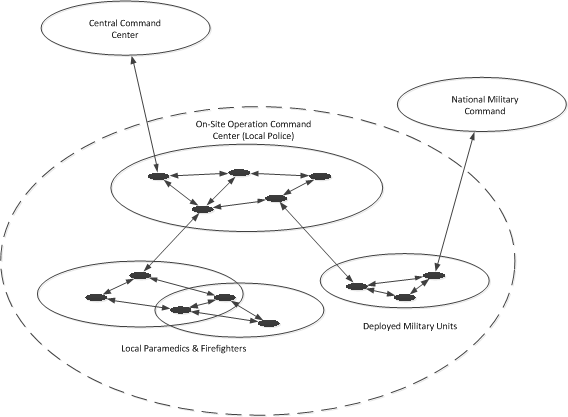
\includegraphics[width=\textwidth]{images/scenario.png}
  	\caption{Scene from scenario with actors from multiple organizations.}
	\label{fig:scenario_networks}
\end{figure}

Choosing whether to merge two networks or not is mainly a security issue. Some
actors might have higher security concerns than others, like the military do not
trust the other actors to merge with their networks, but they might still want
to communicate. This can for example be handled by having certain gateway nodes
being allowed to communicate with nodes outside the network in a controlled
manner.

\subsubsection*{Full Merging}
A \emph{full merging} means that two or more separately built and maintained
networks completely merge so that each node in each of the networks receive
all the routing announcements being sent within the networks. What this
basically means is that the different networks become a single network.

The transition to from multiple to one network is not however, an easy one. Up
until this point the assumption has been that there is only one management node
called \ac{SP} in the network. This will now change. With multiple networks
mering into one there will be multiple \acp{SP} managing the access control of
the network. In the next section having multiple \acp{SP} are discussed in
greater detail.

There is one more major factor which needs to be addressed with full merging of
networks, namely how access control is defined. One now needs to assume that the
\acp{SP} either use the same policy languages to define what rights a node have
been attributed with, or that they have a way of translating these policy
languages so that they can be uniformly understood. For instance, in Section
\ref{subsect:detailed_pc_descr} three special attributes and their values were
used as an example of how a policy might look like:

\begin{itemize}
  \item Role - Node's role in the network
  \item Routing - Whether the node can partake in the routing
  \item Application - Whether the node has access to the application layer
\end{itemize}

Now, these attributes would seem to make sense in most applications of this
system design, but some implementations might even have more attributes. Their
values might also be different, because different networks might have different
needs, for instance the 'role' attribute might have different values depending
on what kind of elements are present in the network. For instance, one network
might have the ``location aware guard nodes'' mentioned earlier in the network
for wormhole protection, while other network do not.

\subsubsection*{Limited Merging}
\emph{Limited merging} is a completely different technique than the one
described above, and probably easier to implement. With limited merging of two or more
networks, the networks stay autonomous with their own (possible) hierarchy, set
of rules, management nodes, and so on. What constitutes the merging is that at
least one node in each network is set up with gateway capabilities, which can
broadcast the existence of another network to the nodes inside its own network.

Rules on the application layer must necessarily still be looked at, as they
should work over the different network, but routing rules and other access
controls can stay hidden between the networks.

\subsubsection*{Internet Gateway}
Similar to limited merging, a node in a network may be given gateway capabilites
to announce Internet access to the network. Because all nodes belong to the same
\ac{MANET} and the management is consistant within this one network, this
capability should be relatively easy to implement. The only thing the reader
should notice is that the policy field within the proxy certificates of the
nodes can now be used to declare whether the node should have Internet access or
not by adding an \emph{Internet attribute} to the policy.

\subsection{Multiple Service Proxies}
Whenever full merging of two secure and managed MANETs happen as described above
two \emph{or more} (!) SPs will end up in the same network (the emphasis on more
is used because one network might have more than one SP). This would be a
challenging task to overcome, for these networks are inherently flat, or
non-hierarchical. Decision making in the network after this point would be
difficult if one network (or specifically on SP) sees itself as more important
than the other.

It is probably better to say that for two networks to fully merge, they should
see themselves as equal counterpart where no network has more rights than the
other, and therefore the \acp{SP} have the same rights as each other. This means
that nodes issued by one \ac{SP}, or said differently one SP's children, are
equally trusted by all other nodes in the network, depending on the restrictions
set in their \acp{PC} of course.

If all the \acp{SP} in the network are considered ``equal'', then they are all
equally trusted to issue new nodes and introduce them to the network. The major
requirement missing for this scheme to happen is that all nodes in the network
now needs to know the public keys for all SPs.

It is likely that not all nodes in the network will ever become a direct
neighbor and therefore not receive the other SPs' \acp{PC0}, but they will meet
nodes signed by those SPs. A way around this problem is to have each \ac{SP} to
once in a while broadcast a digitally signed list to all its children nodes
containing the identities (unique subject names) and public keys for all other
trusted \acp{SP} in the network. Because this list is signed by a known
\ac{SP}, you are able to verify the authenticity of this list and therefore
implicitly verify and trust all nodes issued with PCs from the other SPs.

\section{Experience with OpenSSL}
The experience with OpenSSL has been a challenging one. There is little
documentation available, and only on some segments of the library. Many
functions being used in the implementation of this thesis are undocumented, or
at least not in a freely available documentation. Not to be confused, you can
find most OpenSSL functions in their documentation, but most of those functions
are not explained, many does not explain output and input to functions, and many
functions have unclear names making it a game of ``guessing'' which functions to
use.

Most of the implementation has been understood by looking at a few available
examples online at different sites, some demos within the OpenSSL libraries,
and by asking the online community. For reference, I would personally recommend the
community at \emph{Stack Overflow}\footnote{\url{http://stackoverflow.com}}
rather than the OpenSSL mailinglists\footnote{\url{openssl-dev@openssl.org}}
\footnote{\url{openssl-users@openssl.org}} which have not answered any
questions I raised.

When I've had enough time I've documented the OpenSSL functions used in my
implementation, which can hopefully help someone planning to further implement
on this design, or other designs with similar functionality.

TODO: mention why ECC not used, problems with ECIES algorithm